\PassOptionsToPackage{obeyspaces,spaces}{url}
\documentclass[11pt,a4paper]{article}
\usepackage[margin=2.2cm]{geometry}
\usepackage{amsmath,amssymb}
\usepackage{graphicx}
\usepackage{booktabs}
\usepackage{xcolor}
\usepackage{float}
\usepackage{xurl}
\usepackage[colorlinks=true,linkcolor=blue!50!black,urlcolor=blue!50!black]{hyperref}
\urlstyle{tt}
\newcommand{\code}[1]{\nolinkurl{#1}}
\newcommand{\nptypA}{1.39}
\newcommand{\nplocA}{2.66}
\newcommand{\npwcA}{4.22}
\newcommand{\ncOverMaxdefaultA}{1.93}
\newcommand{\nptypB}{1.50}
\newcommand{\nplocB}{3.28}
\newcommand{\npwcB}{7.74}
\newcommand{\ncOverMaxdefaultB}{3.08}
\newcommand{\nptypC}{1.50}
\newcommand{\nplocC}{3.41}
\newcommand{\npwcC}{9.63}
\newcommand{\ncOverMaxdefaultC}{3.72}
\newcommand{\nptypD}{1.52}
\newcommand{\nplocD}{3.70}
\newcommand{\npwcD}{11.72}
\newcommand{\ncOverMaxdefaultD}{4.42}


\title{The chain-strength prefactor, the coupler range, and shimming\\[4pt]
\large Why $p$ must grow with $N$, where it stops, and how the machine's biases are measured and corrected}
\author{\code{Projects_master_HPQC/scripts/QuantumComputing/Dimod}}
\date{}

\begin{document}
\maketitle
\begin{abstract}
The QPU solves the SK planner problem only after embedding it: each agent becomes a chain of qubits held together by a ferromagnetic coupling $c=p\,J_{\rm rms}\sqrt{N-1}$. This note derives, step by step, a \emph{lower} bound on $p$ (the chains must survive the field of the other $N-1$ agents) and an \emph{upper} bound (after the QPU rescales the problem into its coupler range, the SK couplings must stay above the analogue control error). The lower bound measured on the campaign's instances is $p\approx3$--$4$ at the $N$ that matter, \emph{above} the previous default $1.414$: the intuition that a larger value (``$J=3$'') is needed is correct. The upper bound decreases as $1/\sqrt{N-1}$, so the window closes near $N\approx100$ unless the extended coupler range is used. The second half describes the flux-bias shimming of D-Wave's tutorial, adapted to SK, as implemented in \code{dwave_utils/shimming.py}, and what it measures about the state of the machine.
\end{abstract}
\tableofcontents

%=====================================================================
\section{Setting and notation}
%=====================================================================
The planner's problem for $N$ agents is the SK Hamiltonian without field,
\begin{equation}
H(S)=-\sum_{i<j}W_{ij}S_iS_j,\qquad S_i=\pm1,\qquad W=\tfrac12(J+J^{\mathsf T}),\ W_{ii}=0 .
\end{equation}
For the pure spin glass ($\varepsilon=0$, $J_0=0$) the entries are independent Gaussians,
\begin{equation}
W_{ij}\sim\mathcal N\!\left(0,J_{\rm rms}^2\right),\qquad J_{\rm rms}=\frac{1}{\sqrt N}\qquad(\text{\code{InteractionEnsemble}, }\sigma=1).
\end{equation}
\paragraph{Local field.} The field felt by agent $i$ in configuration $S$ is
\begin{equation}
h_i(S)=\sum_{j\neq i}W_{ij}S_j ,\qquad H(S)=-\tfrac12\sum_i S_ih_i(S).
\end{equation}
For a fixed $S$ independent of $W$ it is a sum of $N-1$ independent terms of variance $J_{\rm rms}^2$:
\begin{equation}
\mathbb E\,h_i^2=(N-1)J_{\rm rms}^2\quad\Longrightarrow\quad |h_i|\sim J_{\rm rms}\sqrt{N-1}=\sqrt{\tfrac{N-1}{N}}\approx1 .
\end{equation}
This is the natural unit for the chain coupling, hence the definition used by the code (\code{uniform_torque_compensation}):
\begin{equation}
\boxed{\,c=p\;J_{\rm rms}\sqrt{N-1}\,}\qquad\Longrightarrow\qquad p=\frac{c}{\text{typical }|h_i|}.
\end{equation}
For our ensemble $c=p\sqrt{(N-1)/N}\approx p$.

\paragraph{Embedding.} Agent $i$ is a chain $C_i$ of $L_i$ qubits (a tree on the chip graph, $L_i\approx N/12+1$ on Zephyr, $N/12+2$ on Pegasus for the clique embeddings). Inside the chain each edge carries the Ising coupling $-c$. Between chains $i$ and $j$ there are $|E_{ij}|\ge1$ physical couplers (1.1--1.2 on average), and $W_{ij}$ is split evenly over them. The physical problem is
\begin{equation}
H_{\rm phys}(s)=-\sum_{i<j}\sum_{(q,q')\in E_{ij}}\frac{W_{ij}}{|E_{ij}|}s_qs_{q'}\;-\;c\sum_i\sum_{(q,q')\in C_i}s_qs_{q'} .
\end{equation}

%=====================================================================
\section{Lower bound: the chains must hold}
%=====================================================================
\subsection{When does a chain break?}
Take chain $i$, all other chains intact. The rest of the problem acts on chain $i$ as a field $h_i$, distributed over its qubits: qubit $q\in C_i$ receives $h_{i,q}$, with $\sum_{q\in C_i}h_{i,q}=h_i$. Suppose the chain points against its field, $S_i h_i<0$ (it does so for a while during the anneal, and in every excited state). Flipping a connected segment $A\subset C_i$ that is cut from the rest by $b(A)$ chain edges changes the energy by
\begin{equation}
\Delta E(A)=\underbrace{2c\,b(A)}_{\text{broken chain edges}}\;-\;\underbrace{2\Big|\sum_{q\in A}h_{i,q}\Big|}_{\text{field energy gained}} .
\end{equation}
The segment that breaks most easily is an end segment of the tree, $b(A)=1$, carrying almost all of the field. The chain is stable against every segment flip if
\begin{equation}
c\;\ge\;\max_A\Big|\sum_{q\in A}h_{i,q}\Big|\;\lesssim\;|h_i| ,
\end{equation}
so a sufficient condition for chain $i$ is $c\ge|h_i|$, and for the whole embedding
\begin{equation}
\boxed{\,c\;\ge\;\max_i|h_i(S)|\quad\text{for the configurations }S\text{ the anneal visits near its end.}\,}
\label{eq:hold}
\end{equation}
At a finite effective temperature $T_{\rm eff}$ at freeze-out, a chain with margin $c-|h_i|$ still breaks with probability $\sim e^{-2(c-|h_i|)/T_{\rm eff}}$: \eqref{eq:hold} is the scale, not a sharp threshold. In units of $J_{\rm rms}\sqrt{N-1}$ the condition reads $p\ge p_\ast(S)=\max_i|h_i(S)|/(J_{\rm rms}\sqrt{N-1})$.

\subsection{Three estimates of the field}
\paragraph{(a) Typical field, $p_{\rm typ}$.} For random $S$, $|h_i|/(J_{\rm rms}\sqrt{N-1})$ is a standard half-normal, with rms 1. At a low-energy state the fields are aligned with the spins and larger: measured at greedy local minima, the rms is $p_{\rm typ}=\nptypA$ at $N=16$, $\nptypB$ at $N=64$, $\nptypC$ at $N=104$.

\paragraph{(b) Largest field at a low-energy state, $p_{\rm loc}$.} What \eqref{eq:hold} needs is the \emph{maximum over the $N$ chains}. At a local minimum $p_{\rm loc}=\max_i|h_i|/(J_{\rm rms}\sqrt{N-1})$ grows slowly with $N$ (extreme value of $N$ roughly Gaussian variables, $\sim\sqrt{2\ln N}$):
\begin{center}
\begin{tabular}{lcccc}
\toprule
$N$ & 16 & 64 & 104 & 160\\
\midrule
$p_{\rm typ}$ (rms field) & \nptypA & \nptypB & \nptypC & \nptypD\\
$p_{\rm loc}$ (largest field, local minimum) & \nplocA & \nplocB & \nplocC & \nplocD\\
$p_{\rm wc}$ (worst case, $\max_i\sum_j|W_{ij}|$) & \npwcA & \npwcB & \npwcC & \npwcD\\
$c/\max|W_{ij}|$ at $p=1.414$ & \ncOverMaxdefaultA & \ncOverMaxdefaultB & \ncOverMaxdefaultC & \ncOverMaxdefaultD\\
\bottomrule
\end{tabular}
\end{center}
(40 instances per $N$, script \code{prefactor_figure.py}.)

\paragraph{(c) Worst case, $p_{\rm wc}$.} Over all configurations, $|h_i|\le\sum_j|W_{ij}|$, reached when every neighbour pulls the same way. With $\mathbb E|W_{ij}|=\sqrt{2/\pi}\,J_{\rm rms}$,
\begin{equation}
\sum_{j\ne i}|W_{ij}|\approx\sqrt{\tfrac2\pi}\,(N-1)J_{\rm rms}
\quad\Longrightarrow\quad
p_{\rm wc}\approx\sqrt{\tfrac2\pi}\sqrt{N-1}\;(\text{mean over }i);\ \text{the max over }i\text{ is a bit larger.}
\end{equation}
Numerically $\sqrt{2/\pi}\sqrt{N-1}=0.798\times\sqrt{103}=0.798\times10.15=8.10$ at $N=104$. This bound guarantees that no configuration breaks a chain. It is far too pessimistic: such configurations have high energy and are not where the anneal ends.

\paragraph{Conclusion of the lower bound.} The relevant scale is $p_{\rm loc}$:
\begin{equation}
p\;\gtrsim\;p_{\rm loc}\approx3\ \ (N\approx30\text{--}60),\qquad\approx3.5\ \ (N\approx100\text{--}180).
\end{equation}
The previous default $p=1.414$ is below this for every $N\ge16$: in low-energy states the most stressed chain is held by less than half of what it needs. Majority vote then repairs the broken chain, but the read is biased. A grid that tests $p$ up to 6 is needed, and \code{coupling-scan} now uses $0.75,1,1.414,2,3,4,6$.

\subsection{What ``$J=3$'' means here}
Two readings are common, and both point the same way.
\begin{enumerate}
\item \emph{Chain coupling three times the largest problem coupling}, $c=3\max|W_{ij}|$. The largest of the $N(N-1)/2$ Gaussians is $\max|W_{ij}|\approx J_{\rm rms}\sqrt{2\ln(N(N-1))}$; at $N=104$: $\sqrt{2\ln 10712}=\sqrt{2\times9.28}=4.31$, so $\max|W|\approx4.31/\sqrt{104}=0.42$ and $c/\max|W|=1.414\times\sqrt{103/104}/0.42\approx3.3$ (measured: \ncOverMaxdefaultC). In this reading the old default was already at ``3'' for $N\gtrsim64$, but below it for small $N$ (\ncOverMaxdefaultA{} at $N=16$).
\item \emph{Chain coupling $\approx3$ in units of the typical field}, i.e.\ $p=3$. This is the $p_{\rm loc}$ scale derived above.
\end{enumerate}
The second reading is the one tied to the physics of chain breaking (fields, not single couplings); for comparison, Teza et al.\ quote chain couplings of 15--20 times the typical problem coupling; here $c/J_{\rm rms}=p\sqrt{N-1}$ is $1.414\times10.15=14$ at $N=104$ for the old default and $3\times10.15=30$ for $p=3$. Their problem is not all-to-all, so the fields on their chains are smaller: the field argument, not the ratio, is what transfers.

%=====================================================================
\section{Upper bound: the SK couplings must stay above the noise}
%=====================================================================
\subsection{Compression by the coupler range}
The QPU accepts couplings in $j_{\rm range}=[-1,1]$. With \code{auto_scale} it divides the whole physical problem by
\begin{equation}
D=\max\Big(c,\ \max_{i<j}\frac{|W_{ij}|}{|E_{ij}|}\Big)=c\qquad\text{as soon as } c\ge\max|W_{ij}|\ (p\gtrsim0.45\text{ at }N=104,\ p\gtrsim0.75\text{ at }N=16).
\end{equation}
The SK coupling $W_{ij}$ is then programmed as $W_{ij}/D$ in total, so its rms on the chip is
\begin{equation}
\frac{J_{\rm rms}}{D}=\frac{J_{\rm rms}}{p\,J_{\rm rms}\sqrt{N-1}}=\boxed{\frac{1}{p\sqrt{N-1}}}.
\end{equation}
Numerically at $N=104$: $1/(1.414\times10.15)=0.070$ for $p=1.414$; $1/(3\times10.15)=0.033$ for $p=3$; $1/(6\times10.15)=0.016$ for $p=6$.

\subsection{Control error}
Every programmed coupling is realised with an error (``integrated control error'', ICE): $J_{qq'}\to J_{qq'}+\delta J_{qq'}$, with $\delta J$ of order $\sigma\approx0.01$--$0.03$ of the range, partly static (calibration, crosstalk), partly fluctuating between programmings. The logical coupling receives the sum of $|E_{ij}|$ such errors, of size $\sigma\sqrt{|E_{ij}|}$. The relative error on each SK coupling is
\begin{equation}
\varepsilon=\frac{\sigma\sqrt{|E_{ij}|}}{J_{\rm rms}/D}=p\,\sigma\sqrt{|E_{ij}|}\sqrt{N-1}.
\end{equation}
Requiring $\varepsilon\le1$ (the instance on the chip still resembles the one we want) gives
\begin{equation}
\boxed{\,p\;\le\;p_{\rm noise}=\frac{1}{\sigma\sqrt{|E|}\sqrt{N-1}}\,}\approx\frac{1}{\sigma\sqrt{N-1}} .
\end{equation}
$\varepsilon\le1$ is necessary, not sufficient: the SK ground state is fragile under small random changes of the couplings (``bond chaos''), so finding the \emph{exact} ground state of the intended instance needs $\varepsilon\ll1$. Numbers at $N=104$ ($\sqrt{N-1}=10.15$):
\begin{center}
\begin{tabular}{lccc}
\toprule
$\sigma$ & 0.01 & 0.02 & 0.03\\
\midrule
$p_{\rm noise}$, range $[-1,1]$ & $1/(0.01\times10.15)=9.9$ & 4.9 & 3.3\\
$p_{\rm noise}$, extended range (Sec.~\ref{sec:ext}) & 19.7 & 9.9 & 6.6\\
\bottomrule
\end{tabular}
\end{center}

\subsection{Field errors grow with $p$ too}
A constant flux offset on qubit $q$ acts as a spurious field $\delta h_q$ (of order $\sigma_h\sim0.01$--$0.05$ of $h_{\rm range}$ on the programmed scale). On a chain of $L$ qubits the logical spin receives $\sum_{q\in C_i}\delta h_q$, between $\sqrt L\,\sigma_h$ (random signs) and $L\,\sigma_h$ (same sign). Compared with the programmed field scale $J_{\rm rms}\sqrt{N-1}/D=1/p$, the relative bias is
\begin{equation}
\beta_i\simeq p\,\sqrt{L_i}\,\sigma_h\quad\text{to}\quad p\,L_i\,\sigma_h .
\end{equation}
It grows with $p$ and with the chain length, and it breaks the $S\to-S$ symmetry of the problem. This is exactly what flux-bias shimming removes (Sec.~\ref{sec:shim}).

%=====================================================================
\section{The window, and what it implies}
%=====================================================================
\begin{figure}[H]
\centering
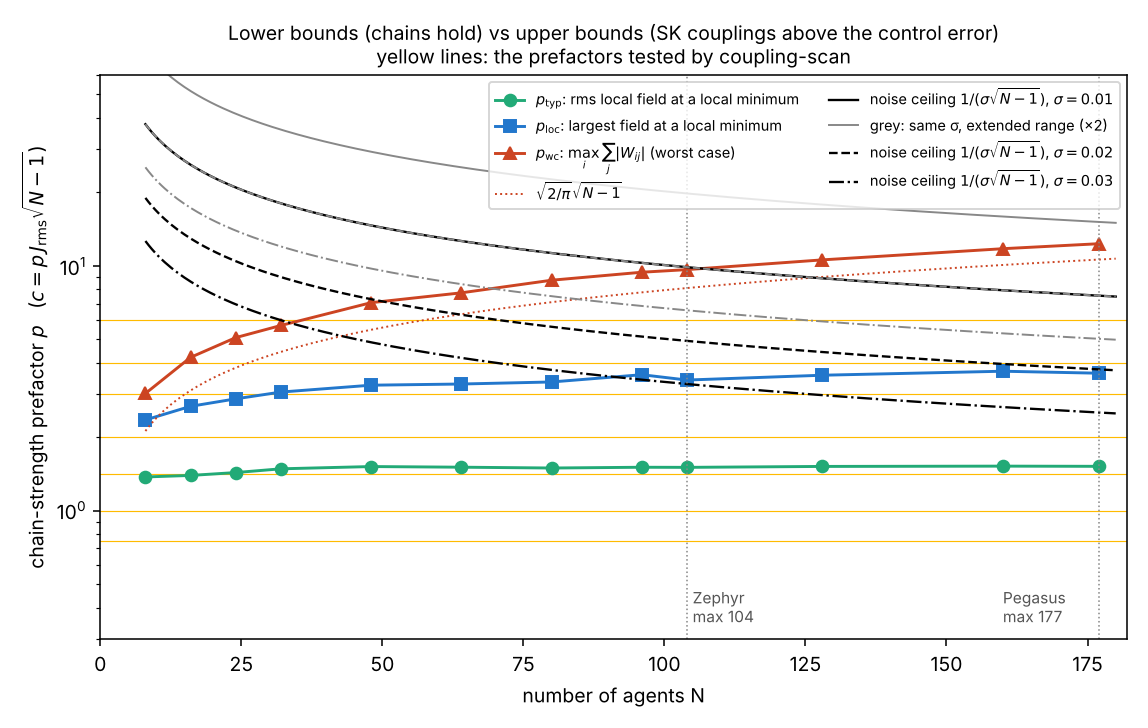
\includegraphics[width=\textwidth]{prefactor_window.png}
\caption{Lower bounds (coloured: the chains hold) and upper bounds (black: the SK couplings are above the control error $\sigma$; grey: the same with the extended coupler range). Yellow: the prefactors tested by \code{coupling-scan}.}
\end{figure}
The usable window is $p_{\rm loc}\lesssim p\lesssim p_{\rm noise}$. Setting $p_{\rm loc}\approx3.5$ equal to $1/(\sigma\sqrt{N-1})$ gives the size where it closes:
\begin{equation}
\sqrt{N_\ast-1}=\frac{1}{3.5\,\sigma}\ \Longrightarrow\ N_\ast=1+\frac{1}{12.25\,\sigma^2}:\quad
\sigma=0.01\to N_\ast\approx 820;\ \ \sigma=0.02\to 205;\ \ \sigma=0.03\to 92 .
\end{equation}
(With the worst-case bound instead, $\sqrt{2/\pi}\sqrt{N-1}=1/(\sigma\sqrt{N-1})$ gives $N_\ast=1+1/(0.798\,\sigma)$: $\approx126$ for $\sigma=0.01$, 64 for $\sigma=0.02$.) So:
\begin{itemize}
\item for $N\lesssim50$ any $p$ in $[3,6]$ is safe on both sides;
\item at $N=104$ on Zephyr the window is $[3.4,\ 3.3\text{--}10]$ depending on the real $\sigma$: it can be narrow, and only the scan tells;
\item at $N=128$--$177$ on Pegasus the extended range (if offered) doubles the room;
\item the ``smallest $p$ with no broken chain'' rule of \code{coupling-scan} picks the lower edge of the window, which is where the SK problem is least compressed.
\end{itemize}

%=====================================================================
\section{Extended coupler range}\label{sec:ext}
%=====================================================================
Advantage QPUs report \code{extended_j_range} $=[-2,1]$: ferromagnetic couplings down to $-2$, with a constraint on the sum of the couplings at each qubit (\code{per_qubit_coupling_range}). Chain couplings are ferromagnetic, the SK couplings stay in $[-1,1]$, so the divisor becomes
\begin{equation}
D_{\rm ext}=\max\Big(\frac{c}{2},\ \max_{W/|E|>0}\frac{W_{ij}/|E_{ij}|}{1},\ \max_{W/|E|<0}\frac{W_{ij}/|E_{ij}|}{-1}\Big),
\end{equation}
and the SK couplings are programmed twice as large: $p_{\rm noise}$ doubles. The code (\code{backends.py}, \code{_scale}) computes $D_{\rm ext}$ itself, sends the scaled problem with \code{auto_scale=False}, checks the per-qubit sum, and falls back to \code{auto_scale} when the solver has no extended range or the check fails. Every result records the mode and the divisor (\code{info.programmed.scaling}); \code{validate} recomputes it.
\begin{verbatim}
python main_simulation.py init --preset full --out results/full3 --extended-j-range
\end{verbatim}
D-Wave notes that couplings in the extended part can be less precise; the scan with and without the option at the same $N$ is the way to see whether it helps.

%=====================================================================
\section{Shimming: measuring and correcting the machine's biases}\label{sec:shim}
%=====================================================================
\subsection{The idea (D-Wave's shimming tutorial)}
The tutorial (\url{https://github.com/dwavesystems/shimming-tutorial}, Chern et al., Front.\ Comput.\ Sci.\ 2023) refines the calibration for a specific problem by using a \emph{symmetry} of that problem: quantities that the symmetry forces to be equal are measured, and the deviations are fed back into small corrections. Two kinds of correction exist:
\begin{itemize}
\item \textbf{flux-bias offsets} $\Phi_q$ per qubit (parameter \code{flux_biases}, units of $\Phi_0$), which cancel spurious fields; the target is a magnetisation that the symmetry fixes;
\item \textbf{coupler adjustments}, which equalise the frustration of couplers that the symmetry makes equivalent (``orbits'').
\end{itemize}

\subsection{Why flux shimming applies to SK, and coupler shimming does not}
With $h=0$, $H(S)=H(-S)$. Every Boltzmann or quantum state of the ideal Hamiltonian is symmetric, so for every physical qubit
\begin{equation}
\langle s_q\rangle=0\qquad\text{exactly.}
\end{equation}
Any measured $m_q=\frac1R\sum_{r=1}^R s_q^{(r)}\neq0$ beyond statistical error is a device bias. Random SK couplings have no symmetry relating different couplers, so there are no orbits and coupler shimming has no target; it is not used.

\subsection{The feedback rule and its convergence}
For small offsets the response is linear: $m_q\approx\chi_q\,(\Phi^{\rm dev}_q+\Phi_q)$, with $\Phi^{\rm dev}_q$ the unknown device offset and $\chi_q>0$ a susceptibility. The update
\begin{equation}
\Phi_q^{(t+1)}=\Phi_q^{(t)}-\alpha_\Phi\,m_q^{(t)}\qquad(\text{tutorial; default }\alpha_\Phi=10^{-5}\,\Phi_0)
\end{equation}
gives for the residual $e^{(t)}=\Phi^{\rm dev}+\Phi^{(t)}$
\begin{equation}
e^{(t+1)}=(1-\alpha_\Phi\chi)\,e^{(t)}-\alpha_\Phi\,\eta^{(t)},
\end{equation}
where $\eta$ is the shot noise of $m_q$. It converges geometrically if $0<\alpha_\Phi\chi<2$, with time constant $1/(\alpha_\Phi\chi)$ iterations. At stationarity the residual jitters with variance
\begin{equation}
\mathrm{Var}\,e=\frac{\alpha_\Phi^2\,\mathrm{Var}\,\eta}{1-(1-\alpha_\Phi\chi)^2}\approx\frac{\alpha_\Phi\,\mathrm{Var}\,\eta}{2\chi}\qquad(\alpha_\Phi\chi\ll1):
\end{equation}
a small $\alpha_\Phi$ averages more reads, a large one converges faster.

\paragraph{The shot-noise floor.} In a low-energy SK state each read picks one of the two mirror states, so $s_q=\pm1$ with equal probability and
\begin{equation}
\mathrm{Var}\,m_q=\frac1R\ \Longrightarrow\ \text{rms }m_q\approx\frac{1}{\sqrt R}=0.1\ \text{for }R=100 .
\end{equation}
A measured rms $|m_q|$ near $1/\sqrt R$ is \emph{noise, not bias}; only the excess above it is device bias. Over $T$ iterations the offsets average $TR$ reads, so biases down to $\sim1/\sqrt{TR}$ ($=0.018$ for $T=30$, $R=100$) are corrected. \code{shim_history.png} draws the $1/\sqrt R$ line.

\paragraph{Qubit or chain level.} At the \emph{qubit} level (tutorial) each qubit is corrected by its own $m_q$. At the \emph{chain} level (Teza et al., Methods, Eq.~8) all qubits of chain $i$ are corrected by the chain's mean $m_i$: unbroken chains have $m_q=m_i$ for every $q$, and the chain-level estimate averages $L_i$ qubits, but cannot see a bias that varies along a chain. Option \code{--level qubit|chain}.

\paragraph{Gauges.} At every iteration the instance is transformed by random signs $g_i$: $W_{ij}\to g_ig_jW_{ij}$, $S_i\to g_iS_i$. The physics is identical, but the coupler errors now add to the qubit fields with random signs from one iteration to the next. The feedback then learns biases of the \emph{device}, not of one instance's coupler errors. Option \code{--no-gauge} disables it.

\subsection{What it tells about the state of the machine}
The shim history (\code{shims/<backend>/history.json}) records per iteration: rms and max $|m_q|$, rms chain magnetisation, rms and max offset, chain-break fraction, best energy, QPU time, chip-graph fingerprint, problem id. Read it as follows:
\begin{itemize}
\item rms $m_q$ at the first iteration well above $1/\sqrt R$: the device is biased for this embedding; the excess is its size;
\item rms $m_q$ falling to $1/\sqrt R$: the bias is corrected; the offsets $\Phi_q$ are a map of the device's flux offsets on the qubits used;
\item rms $m_q$ not falling: $\alpha_\Phi$ too small (raise it) or bias drifting faster than the feedback;
\item offsets of a later session very different from today's, or a different \code{graph_sha1}: the chip was recalibrated; shim again;
\item \code{--alpha-phi 0}: a pure diagnostic, nothing changed, only the biases measured.
\end{itemize}
The offsets are stored in \code{shims/<backend>/fbos.json} and, with the default \code{--apply}, used by every later \code{qpu} call of that back-end (\code{flux_biases}, \code{flux_drift_compensation=True}); each result records how many offsets were applied and their rms (\code{info.flux_biases}).

\subsection{Commands and cost}
\begin{verbatim}
python main_simulation.py shim --out results/full2 --backend qpu:zephyr:clique  --N 64 --check
python main_simulation.py shim --out results/full2 --backend qpu:zephyr:clique  --N 64 --iterations 30 --budget-seconds 1.5
python main_simulation.py shim --out results/full2 --backend qpu:pegasus:clique --N 64 --iterations 30 --budget-seconds 1.5
\end{verbatim}
One iteration with 100 reads at $N=64$ is $\approx15.8\ \text{ms}+100\times0.2\ \text{ms}\approx37$ ms; 30 iterations $\approx1.1$ s per QPU. The offsets are learned for the qubits of the clique embedding of that $N$; larger $N$ use a superset of qubits, and the qubits not shimmed get no offset. To shim at the largest size, run at $N=104$ (Zephyr) or $N=160$ (Pegasus), $\approx$1.5--2 s each.

%=====================================================================
\section{Recommended order with the remaining budget}
%=====================================================================
\begin{enumerate}
\item \code{coupling-scan} with $p\in\{0.75,1,1.414,2,3,4,6\}$ at $N=8,16,\dots,48$ and 104, both QPUs: $7\times7\times2=98$ calls of $\approx15.8\ \text{ms}+200\times0.2\ \text{ms}\approx55$ ms, $\approx5.4$ s. Expect the chosen $p$ to rise from $\approx2$ at small $N$ to $\approx3$--$4$.
\item Shimming at the largest $N$ of each QPU, 30 iterations: $\approx3$--$4$ s in total.
\item Optionally the same scan at $N=104$ with \code{--extended-j-range} (a second campaign directory), $p\in\{3,4,6\}$: $<1$ s.
\item The main run with the chosen table, shims applied.
\end{enumerate}
\end{document}
